% Date : April 1, 2020
% Author : 
% Subhankar Mishra
% School of Computer Sciences 
% NISER

\documentclass[12pt,a4paper]{report}
\setlength{\oddsidemargin}{0.25in}
\setlength{\evensidemargin}{0.15in}
\setlength{\topmargin}{0.3in}
\setlength{\textwidth}{6.0in}
\setlength{\textheight}{8.5in}
\usepackage{amsmath,amssymb}
\usepackage{graphics}
\usepackage{lscape,graphicx}
\usepackage{amsfonts}
\usepackage{longtable}
\usepackage{epsfig}
\usepackage{float}
\usepackage{rotating}

\usepackage{fancyhdr}
\usepackage{listings}
\usepackage{xcolor}

\definecolor{codegreen}{rgb}{0,0.6,0}
\definecolor{codegray}{rgb}{0.5,0.5,0.5}
\definecolor{codepurple}{rgb}{0.58,0,0.82}
\definecolor{backcolour}{rgb}{0.95,0.95,0.92}

\lstdefinestyle{mystyle}{
	backgroundcolor=\color{backcolour},   
	commentstyle=\color{codegreen},
	keywordstyle=\color{magenta},
	numberstyle=\tiny\color{codegray},
	stringstyle=\color{codepurple},
	basicstyle=\ttfamily\footnotesize,
	breakatwhitespace=false,         
	breaklines=true,                 
	captionpos=b,                    
	keepspaces=true,                 
	numbers=left,                    
	numbersep=5pt,                  
	showspaces=false,                
	showstringspaces=false,
	showtabs=false,                  
	tabsize=2
}

\lstset{style=mystyle}
\usepackage{hyperref}
\hypersetup{
	colorlinks=true,
	linkcolor=blue,
	filecolor=blue,
	citecolor = blue,      
	urlcolor=cyan,
}
\usepackage{siunitx}
\DeclareSIUnit \h {\mbox{$h$}}
\DeclareSIUnit \parsec {pc}
\usepackage[
backend=biber,
citestyle=authoryear,
bibstyle=science,
]{biblatex}
\AtEveryCitekey{\clearfield{title}}
\addbibresource{reference.bib}
\setlength{\headheight}{15pt}
\usepackage[titletoc]{appendix}
\usepackage[english]{babel}
\addto{\captionsenglish}{\renewcommand{\bibname}{References}}

\usepackage{titlesec}
\titlespacing*{\chapter}{0pt}{0pt}{0pt}
\titleformat{\chapter}[display]{\normalfont\huge\bfseries}{\chaptertitlename\ \thechapter}{20pt}{\Huge}

%%%%%%%%%%%%%%%%%%%%%%%%%%%%%%%%%%%%%%%%%%
%%%  macro for margin change
\newenvironment{changemargin}[2]{%
\begin{list}{}{%
%\setlength{\topsep}{0pt}%
\setlength{\leftmargin}{#1}%
\setlength{\rightmargin}{#2}%
%\setlength{\listparindent}{\parindent}%
%\setlength{\itemindent}{\parindent}%
%\setlength{\parsep}{\parskip}%
}%
\item[]}{\end{list}}
%%%%%%%%%%%%%%%%%%%%%%%%%%%%%%%%%%%%%%%%%%

\begin{document}
\begin{changemargin}{0cm}{0cm}
\thispagestyle{empty}
\baselineskip25pt
\begin{center}
{\Large {\bf STACKING OF VOID GALAXIES}}\\
\end{center}

\vfill
\baselineskip15pt
\begin{center}
{\em A Project Report submitted} \\
in Fulfilment of the Requirements \\
for the completion of \
\vskip .30\baselineskip
{\large{\bf SUMMER INTERNSHIP}}
\end{center}
\baselineskip25pt

\vfill
\begin{center} {\bf {\em by}} \\
{\large{\bf MAITREY SHARMA}} \\
\end{center}

\vfill
\begin{center}
\begin{figure}[h!]
\centering

\includegraphics[scale=0.2]{logo1.jpg}
% Reference for the Logo: Student Forms | NISER https://www.niser.ac.in/forms/academic/LaTexTemplate_MScThesis.zip
\end{figure}
 {\bf {\em to the }} \\
{\bf {\large School of Physical Sciences}} \\
{\bf {\large National Institute of Science Education and Research}} \\
{\bf Bhubaneswar} \\
{\bf \today} 
\end{center}
\end{changemargin}



\pagenumbering{roman}
\baselineskip=20pt
%
\begin{center}
{\large {\bf DEDICATION (OPTIONAL)}} 
\end{center}


\begin{center}
{\bf DECLARATION}
\end{center}

I hereby declare that I am the sole author of this report in  fulfillment of the requirements for Summer Internship from National Institute of Science Education and Research (NISER). I authorize NISER to lend this report to other institutions or individuals for the purpose of scholarly research.

\vskip1.0in

\hspace*{3.5in} {Signature of the Student} \\
\hspace*{3.5in} {Date:}

\vskip1.0in
\vskip1.0in

The work reported in the report entitled .......................................................  was carried out under my supervision, in the school of ............................................... at NISER, Bhubaneswar, India.

\vskip1.0in

\hspace*{3in} {Signature of the project supervisor} \\
\hspace*{3in} {School:}\\
\hspace*{3in} {Date:}
%\include{stat}
%\include{cert1}
%\begin{center}
{\bf ACKNOWLEDGEMENTS}
\end{center}

I wish to thank xxx......


\begin{center}
{\large {\bf  ABSTRACT }}

In this work we first discuss the cosmological voids and the galaxies that are present in these crucial components of the Cosmic Web. We work through the arguments that solidify the importance of void galaxies to galaxy formation and the effects of their cosmological neighborhood on galaxy evolution. We discuss the cosmic microwave background radiation and how its anisotropies can be probed in void galaxies, with our interest being on the thermal Sunyaev-Zeldovich effect. After the theoretical basis we obtain a publicly available void galaxy catalog and create a filter to remove wall galaxies within a void so that we can increase the signal-to-noise ratio in our stacking techniques.
\end{center}  


    


\clearpage
\fancyfoot{}      % Delete current footer settings

\pagestyle{fancyplain}
 \renewcommand{\chaptermark}[1]{\markboth{\thechapter\ #1}{\thechapter\ #1}} % remember chapter title
 \lhead[\fancyplain{}{}]{\fancyplain{}{}}
 \rhead[\fancyplain{}{}]{\fancyplain{}{\em\leftmark }}
 \renewcommand{\headrulewidth}{0.3pt}
 \cfoot{\rm\thepage} % page number

\baselineskip=12pt
\tableofcontents
\clearpage
%\listoffigures
\clearpage
%\listoftables 
\clearpage
\pagenumbering{arabic}
\baselineskip=15pt
\chapter{\label{intro}Introduction}
Universe is amazing and vast
\setcounter{equation}{0}
\setcounter{table}{0}
\setcounter{figure}{0}
%\baselineskip 24pt


    




\chapter{\label{method}Methods}

\setcounter{equation}{0}
\setcounter{table}{0}
\setcounter{figure}{0}

\section{Distance Measures in Cosmology}
Cosmological distances require special considerations as effects of general relativity, which is, expansion of spacetime becomes substantial that objects are very heavily redshifted. Hubble's law, also known as the Hubble–Lemaître law, is the observation in physical cosmology that galaxies are moving away from Earth at speeds proportional to their distance.
\par 
The Hubble constant $ H_0 $ is the constant of proportionality between recession speed $ v $ and distance $ d $ in the expanding Universe;
\begin{equation}
	v = H_0 d
\end{equation}
The subscripted ``0'' refers to the present epoch because in general $ H $ changes with time. The dimensions of $ H_0 $ are inverse time, but it is usually written
\begin{equation}
	H_0 = \SI{100}{\h \kilo \meter \per \second \per \mega \parsec}
\end{equation}
where $ h $ is a dimensionless Hubble constant and is often introduced to denote the ``present'' cosmology. We further define the Hubble distance as
\begin{equation}
	d_H \equiv \dfrac{c}{H_0} = \SI{9.26e25}{\per \h \metre}
\end{equation}
Then there are the density parameters $ \Omega_r $ (radiation density), $\Omega_m$ (matter density), $\Omega_{\Lambda}$ (dark energy density) and $\Omega_k$ (curvature density) which together define the dimensionless Hubble parameter $ E(z) $. All these quantites can be expressed as function of redshift $ z $ and summarised in the following equation;
\begin{equation}
	E (z) = \dfrac{H(z)}{H_0} = \sqrt{\Omega_r(1+z)^4 + \Omega_m(1+z)^3 + \Omega_k(1+z)^2 + \Omega_{\Lambda}}
\end{equation} 
All of these form the basis of a more convenient way of dealing with distances in cosmology: comoving distances. \textit{Proper distance} roughly corresponds to where a distant object would be at a specific moment of cosmological time, which can change over time due to the expansion of the universe. \textit{Comoving distance} factors out the expansion of the universe, giving a distance that does not change in time due to the expansion of space. Mathematically, comoving distance $ d_C $ is given by
\begin{equation}
	d_C(z) = d_H \int_0^z \dfrac{dz'}{E(z')}
\end{equation}
\section{Implementation}
The first goal is to create a filter to increase the signal-to-noise ratio of the eventual stacking that will be done. The galaxies which are too near the walls of the voids, the wall galaxies are to be removed. For this following steps were taken:
\par 
Using the catalogues made available by \citeauthor{pan_cosmic_2012} (\cite*{pan_cosmic_2012}), data was imported for void centres (using \verb|public_void_catalog.txt|) and void galaxies (using the \newline \verb|maglim_void_galaxies.txt|). To get the coordinates of void centres from here, the columns of $ x $, $ y $, $ z $ distances were used and column $ r $ was used to get void radius. To take the cosmology into account, the radius $ r $ by $ 0.7 $ (in accordance with the data). To find the comoving distances to void galaxies and void centres, we use $ d = \sqrt{x^2 + y^2 + z^2} $ where $ (x, y, z) $ denote coordinates. The obtained comoving distances are now multiplied by $ 0.7 $ to take cosmology into account. After this, a simple program was written using the Astropy package\footnote{\url{http://www.astropy.org}} for Python, which basically calculates distance of every void centre and galaxy pair and returns the galaxy number corresponding to the void number which satisfies a given fractional distance condition (eg. all void galaxies which are at a distance from $ 0.5r $ where $ r $ is the void radius).
\section{The code}
The Python code, which implements the process described in the last section is given here:
\begin{lstlisting}[language=Python, caption=Code for filtering wall galaxies]
	import numpy as np
	from astropy.coordinates import SkyCoord
	from astropy import units as u
	
	# importing void and galaxy data
	data_gal = np.loadtxt('maglim_void_galaxies.txt')
	data_void = np.loadtxt('public_void_catalog.txt')
	
	# stripping the data
	ra_void = data_void[:, 0]
	dec_void = data_void[:, 1]
	ra_gal = data_gal[:, 0]
	dec_gal = data_gal[:, 1]
	
	
	x_void = data_void[:, 2] 
	y_void = data_void[:, 3]
	z_void = data_void[:, 4]
	void_radius = data_void[:, 5]*0.7
	
	x_gal = data_gal[:, 6]
	y_gal = data_gal[:, 7]
	z_gal = data_gal[:, 8]
	
	#following code to check if comoving distances are same as given in catalog
	cmvdist_gal = np.sqrt(x_gal**2+y_gal**2+z_gal**2)*0.7
	cmvdist_void  = np.sqrt(x_void**2+y_void**2+z_void**2)*0.7
	
	#the main part of the code
	for i in range(len(coord_void)):#range(len(coord_void)):
		c2 = SkyCoord(ra=ra_gal*u.degree, dec=dec_gal*u.degree, distance=cmvdist_gal*u.Mpc)
		c1 = SkyCoord(ra=ra_void[i]*u.degree, dec=dec_void[i]*u.degree, distance=cmvdist_void[i]*u.Mpc)
		dist = c1.separation_3d(c2)
		frac_dist = dist.value/void_radius[i]
		a = np.where(frac_dist <= 0.5) #this is the case for 0.5r
		print("For void number #",i+1, a[0]+1)
	
\end{lstlisting}
%\baselineskip 24pt


    




\chapter{\label{results}Results and Discussion}
After implementing the code, the filter can be generated as per user's requirements. Some plots are included with did not use the filter but represent the results which are obtained by stacking the void galaxies. MILCA refers to Modified Internal Linear Component Algorithm (\cite{hurier_milca_2013}), which is a internal linear combination (ILC) method used to extract the CMB emission from the WMAP multifrequency data courtesy projects like the Planck survey. NILC stands for Needlet Internal Linear Combination (\cite{remazeilles_cmb_2011}), a different technique used for same purpose.
\begin{figure}[h!]
	\centering
	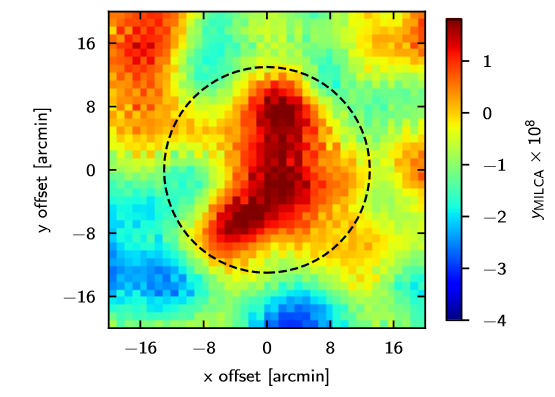
\includegraphics{fig2.png}
	\caption{The normalized stacked $ y $ MILCA map at void galaxy locations at all z in our sample over $ 51\% $ sky mask.}
\end{figure}
\begin{figure}[h!]
	\centering
	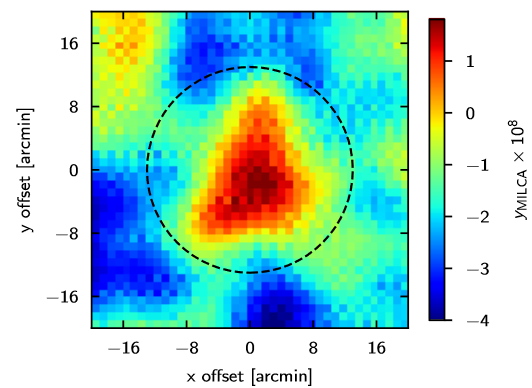
\includegraphics{fig3-1.png}
	\caption{The normalized stacked $ y $ MILCA map at void galaxy locations at $ z > 0.04 $ in our sample over $ 51\% $ sky mask.}
\end{figure}
\begin{figure}[h!]
	\centering
	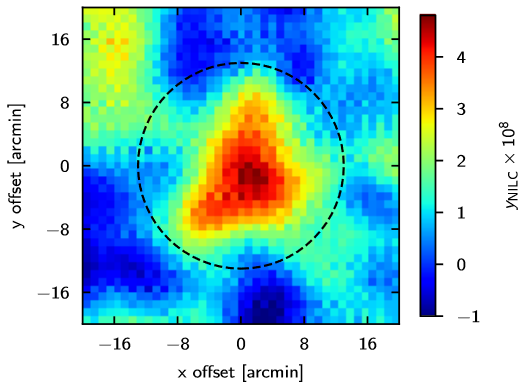
\includegraphics{fig3-2.png}
	\caption{The normalized stacked $ y $ NILC map at void galaxy locations at $ z > 0.04 $ in our sample over $ 51\% $ sky mask.}
\end{figure}
Using the filter, similar stacking plots can be obtained. The filtering will aid in removing unwanted galaxies, that are too near the void walls. 
\setcounter{equation}{0}
\setcounter{table}{0}
\setcounter{figure}{0}
%\baselineskip 24pt


    




%\chapter{\label{summary}Summary and Conclusions}

\setcounter{equation}{0}
\setcounter{table}{0}
\setcounter{figure}{0}
%\baselineskip 24pt


    




%%\clearpage
%\addcontentsline{toc}{chapter}{Appendices}
\begin{appendices}
\chapter{\label{appendix} Eras of Thermalization}
\chapter{\label{key} HealPix}
\end{appendices}


\setcounter{equation}{0}
\setcounter{table}{0}
\setcounter{figure}{0}
%\baselineskip 24pt


    




%\newline
Birkinshaw M. 1999. Physics Reports. 310(2–3):97–195
\newline
Emritte MS, Colafrancesco S, Marchegiani P. 2016. J. Cosmol. Astropart. Phys. 2016(07):031–031
\newline
Fielding D, Quataert E, McCourt M, Thompson TA. 2017. Mon. Not. R. Astron. Soc. 466(4):3810–26
\newline
Haider M, Steinhauser D, Vogelsberger M, Genel S, Springel V, et al. 2016. Mon. Not. R. Astron. Soc. 457(3):3024–35
\newline
Hogg DW. 2000
\newline
Hurier G, Macías-Pérez JF, Hildebrandt S. 2013. A&A. 558:A118
\newline
Kreckel K, Platen E, Aragón-Calvo MA, van Gorkom JH, van de Weygaert R, et al. 2012. The Astronomical Journal. 144(1):16
\newline
Luzzi G, Shimon M, Lamagna L, Rephaeli Y, De Petris M, et al. 2009. ApJ. 705(2):1122–28
\newline
Pan DC, Vogeley MS, Hoyle F, Choi Y-Y, Park C. 2012. Monthly Notices of the Royal Astronomical Society. 421(2):926–34
\newline
Remazeilles M, Delabrouille J, Cardoso J-F. 2011. Monthly Notices of the Royal Astronomical Society. 410(4):2481–87
\newline
Singari B, Ghosh T, Das M, Ma Y-Z, Tanimura H. , p. 6
\newline
Sunyaev RA, Zeldovich YaB. 1970. Astrophys Space Sci. 7(1):3–19
\newline
Tanimura H, Aghanim N, Douspis M, Beelen A, Bonjean V. 2019. A&A. 625:A67
\newline
Tumlinson J, Peeples MS, Werk JK. 2017. Annu. Rev. Astron. Astrophys. 55(1):389–432
\newline
van de Weygaert R, Kreckel K, Platen E, Beygu B, van Gorkom JH, et al. 2011. , pp. 17–24
\newline
van de Weygaert R, Platen E. 2011. Int. J. Mod. Phys. Conf. Ser. 01:41–66
%}
\nocite{*}

\printbibliography
\addcontentsline{toc}{chapter}{Bibliography}
\end{document}
